91. \begin{figure}[ht!]
\center{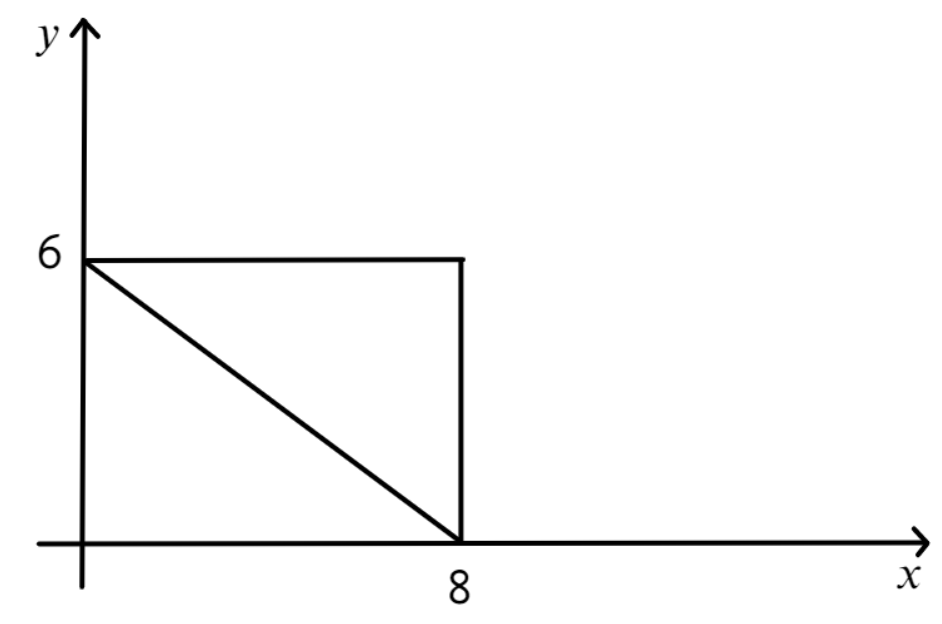
\includegraphics[scale=0.35]{g9-90.png}}
\end{figure}\\
Рассматриваемый треугольник является прямоугольным, поэтому центр его описанной окружности --- это середина гипотенузы. Её ордината равна $(6+0):2=3.$\newpage\noindent
